\documentclass[11pt,a4paper]{article}
\usepackage[margin=1in]{geometry}
\usepackage{amsmath,amssymb}
\usepackage{graphicx}
\usepackage{booktabs}
\usepackage{xcolor}
\usepackage[numbers,sort&compress]{natbib}
\usepackage{caption}
\usepackage{subcaption}
\usepackage[colorlinks=true,linkcolor=blue!55!black,urlcolor=blue!55!black,
            citecolor=blue!55!black,
            pdftitle={The Lavender Flash of August 9th},
            pdfauthor={CMU Skyline Monitor (Simon DeDeo, with Claude)},
            pdfsubject={Colorimetric closure test of lightning emission through a fixed-exposure camera},
            pdfkeywords={lightning spectroscopy, colorimetry, nitrogen fixation, N2+ first negative, urban meteorology}]{hyperref}
\usepackage{microtype}

\newcommand{\code}[1]{\texttt{\small #1}}
\newcommand{\Ntp}{N$_2^+$}

\title{\bfseries The Lavender Flash of August 9th\\[0.4em]
  \large\mdseries Lightning colorimetry from plasma physics to webcam Bayer}
\author{CMU Skyline Monitor --- \code{pandr} ---
  \href{https://proofsandreasons.io}{\code{proofsandreasons.io}}\thanks{Operated by
Simon DeDeo (Carnegie Mellon University). Analysis and code developed with AI
assistance (Claude, Anthropic); the human operator is responsible for all claims,
citations and errors.}}
\date{2026-08-11 (v3)}

\begin{document}
\maketitle

\begin{abstract}
\noindent
At 00:11~EDT on 9 August 2026, a fixed-exposure skyline camera in Pittsburgh
recorded a single frame in which an overcast midnight sky turned pale lavender:
sky-band mean $(R,G,B)=(172,170,223)$ against a sodium-amber baseline of
$(22,19,7)$. We treat this as a closure test: can the color be predicted from
the physics of lightning emission, propagated through cloud, air, and the
camera's color pipeline? A three-component spectral model---a 30\,000~K
continuum standing in for free--free and free--bound emission, N\,\textsc{ii}
and hydrogen Balmer lines, and the \Ntp{} first-negative band system---is
integrated against approximate Bayer sensitivities with daylight (5600~K)
white-balance gains, the configuration the instrument locks by design. The
measured chromaticity is reproduced to one digital number by a mixture of
$\sim$20\% continuum, 65\% atomic-line, and 12--21\% molecular-band energy,
the molecular range bracketed by the optically-thick (Planck) and
optically-thin (Kramers) continuum limits. Atomic lines and continuum alone
cannot reach the observed blueness: the violet \Ntp{} contribution is
\emph{required} under either limit.
We detail the emission components and how the degeneracy could be broken,
connect the \Ntp{} bands to lightning's role in nitrogen fixation, and close
with the color theory of a purple no eye witnessed.
\end{abstract}

\begin{figure}[h]
  \centering
  \begin{subfigure}[t]{0.325\textwidth}
    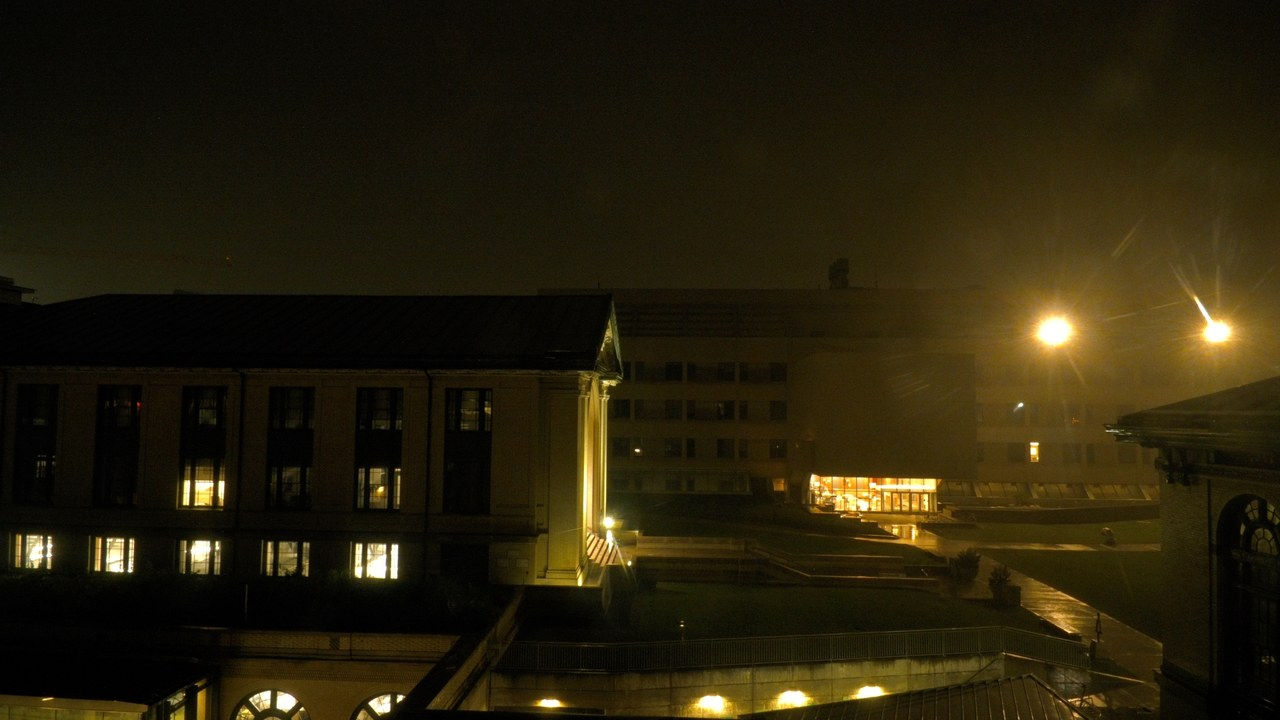
\includegraphics[width=\textwidth]{frame_before.jpg}
    \caption*{\footnotesize 00:06 EDT}
  \end{subfigure}\hfill
  \begin{subfigure}[t]{0.325\textwidth}
    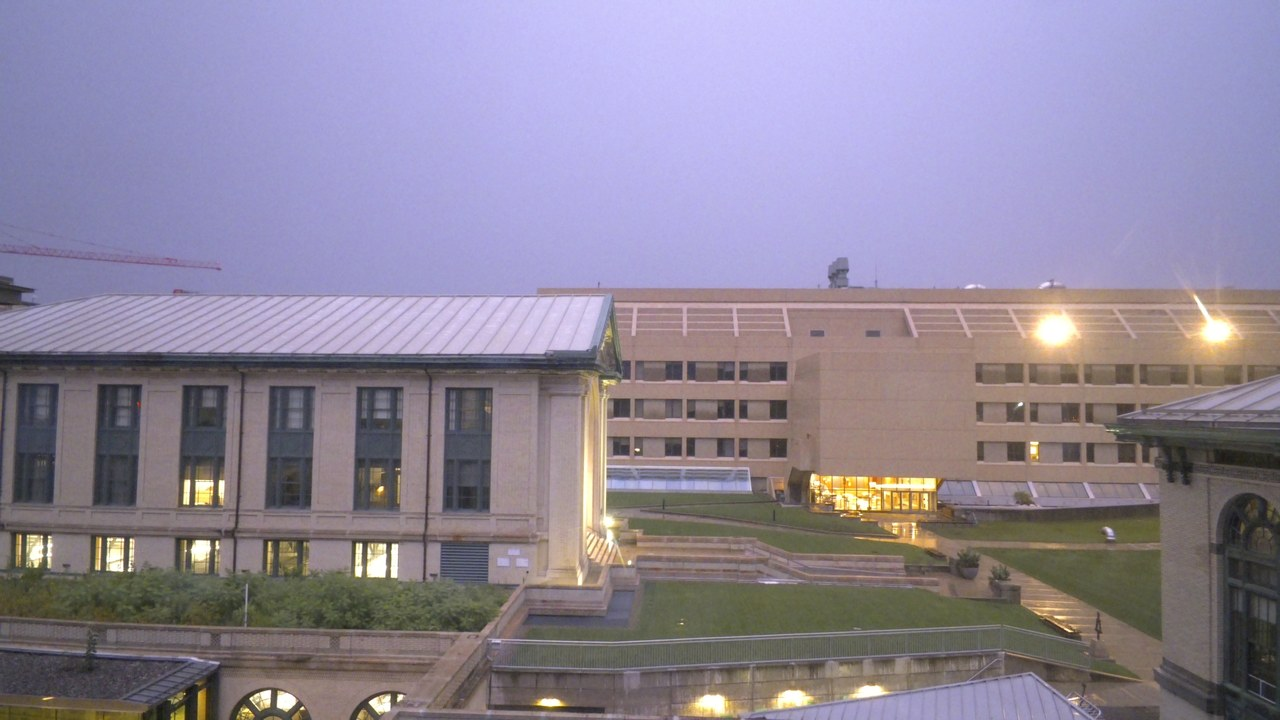
\includegraphics[width=\textwidth]{frame_flash.jpg}
    \caption*{\footnotesize 00:11 EDT --- the flash}
  \end{subfigure}\hfill
  \begin{subfigure}[t]{0.325\textwidth}
    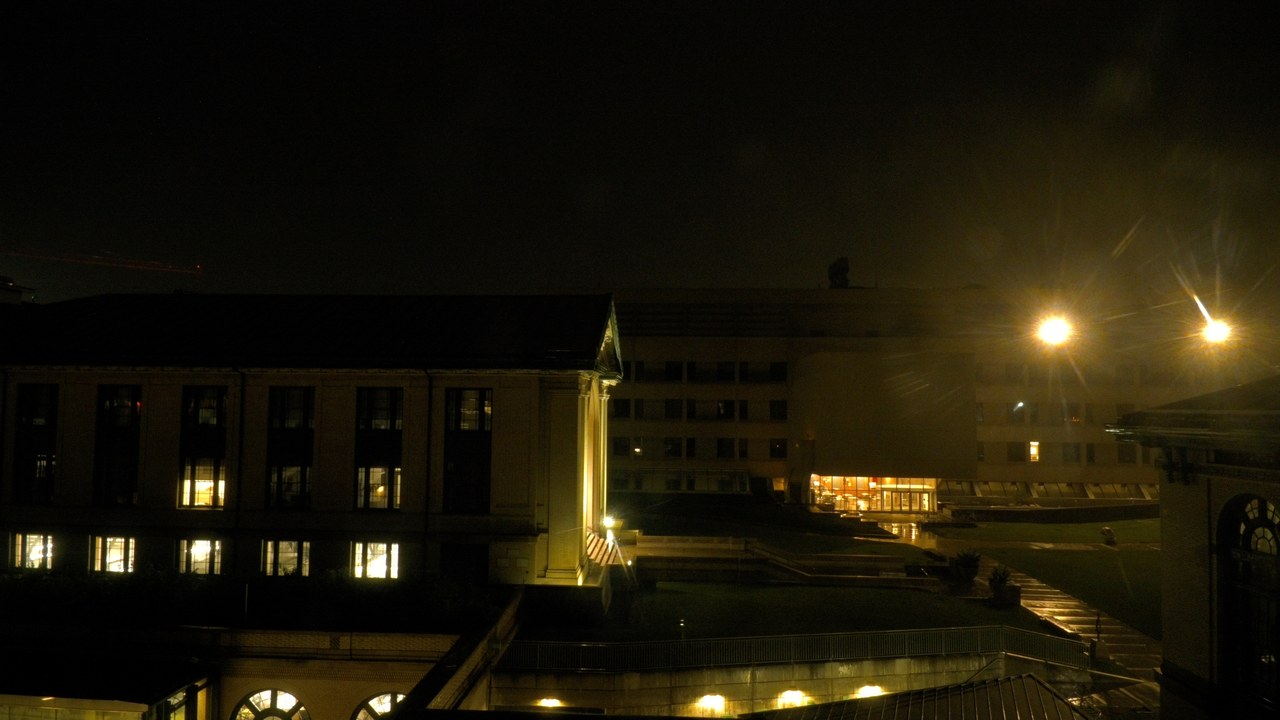
\includegraphics[width=\textwidth]{frame_after.jpg}
    \caption*{\footnotesize 00:17 EDT}
  \end{subfigure}
  \caption{Three consecutive fixed-exposure reference frames (100~ms,
  gain and white balance locked), night of 8--9 August 2026. Fixed light
  sources are unchanged across the triplet (lit windows $162\to174\to161$;
  lamp cores $242\to250\to243$), ruling out an exposure or gain excursion:
  the middle frame records real, additive, sky-borne light.}
  \label{fig:frames}
\end{figure}

\section{The observation}
The monitor captures a radiometric reference frame of the Carnegie Mellon
skyline every five minutes with sun-elevation-keyed manual exposure, fixed
gain, and fixed 5600~K white balance. On the night in question the log shows
one anomalous sample: full-frame brightness 138.7 (neighbors 19--37) and
sky color \code{\#b9b5ed}. The 100~ms exposure integrated one or more strokes
of a flash whose light, diffused by the overcast deck, illuminated the scene
to twilight levels (Fig.~\ref{fig:frames}). Two later samples (00:33, 00:39)
show weak blue excursions consistent with more distant flashes. Linearizing
the sRGB-encoded means \citep{iec1999} and subtracting the baseline frame
gives the flash-only linear color
\begin{equation}
  (r,g,b)_{\rm flash} = (0.405,\,0.396,\,0.736), \qquad
  R/G = 1.023,\quad B/G = 1.860 .
  \label{eq:meas}
\end{equation}
Blue far above green, red slightly above green: pale lavender. The question
is whether these two ratios are quantitatively consistent with what lightning
emits.

\section{Physics: the anatomy of the emission}
\label{sec:physics}

\subsection{The channel}
A return stroke drives $\sim$30~kA through a centimeter-scale channel,
shock-heating it to a peak of 28\,000--31\,000~K within microseconds
\citep{prueitt1963,orville1968,rakovuman2003}. For the first microseconds the
channel is optically thick and radiates as a quasi-blackbody; it becomes
transparent (except in strong line cores) as it expands and cools
\citep{uman1965}. Electron densities inferred from the Stark broadening of
H$\alpha$ start near $10^{18}\,\mathrm{cm^{-3}}$ and fall an order of
magnitude within tens of microseconds \citep{uman1964}; the temperature
falls through $\sim$20\,000~K on the same timescale and reaches
$\sim$10\,000~K by 50~$\mu$s \citep{orville1968}. A camera exposure of
100~ms therefore integrates the \emph{entire} thermodynamic history of every
stroke it catches---and a typical cloud-to-ground flash contains 3--5 strokes
spread over 200--300~ms \citep{rakovuman2003}, so the frame may hold several.
This time-integration is the physical origin of the mixture model below, and
(\S\ref{sec:degeneracy}) of its degeneracy.

\subsection{The continuum}
Beneath the lines lies a genuine continuum, dominated not by blackbody
emission but by two free-electron processes in the transparent plasma:
free--free bremsstrahlung, electrons scattering in ion fields, and
free--bound radiative recombination, electrons captured onto H$^+$, N$^+$,
and O$^+$ \citep{uman1965,zeldovich1966,orvillehenderson1984}. Recombination
continua carry series-edge structure rather than a Planck shape: the hydrogen
Balmer continuum jumps at 364.6~nm, just outside the camera passband, while
the Paschen continuum (captures to $n=3$) spans the entire visible band with
its edge at 820~nm and an intensity rising toward the blue. The
\emph{slope} of this continuum depends on the channel's opacity state. While
optically thick (the first microseconds), it radiates a Planck curve---an
effective $\lambda^{-3.5}$ across our band at 30\,000~K. Once transparent,
free--free and free--bound emission follow the much flatter Kramers form,
$\varepsilon_\lambda \propto \lambda^{-2} e^{-hc/\lambda k T}$, an effective
$\lambda^{-1.1}$: distinctly redder at the same temperature. The
time-integrated continuum is an unknown blend of the two phases, so we fit
the mixture model with each limit and let them bracket the answer
(\S\ref{sec:fit}). In time-resolved spectra
the continuum flashes brightest in the first few microseconds, when the
channel is hottest and densest \citep{orville1968}; its share of the
\emph{time-integrated} visible energy is the model's $w_c$.

\subsection{The atomic lines}
At channel temperatures ($kT \simeq 2.6$~eV) collisional excitation
populates levels tens of eV up in singly ionized nitrogen, and the
N\,\textsc{ii} spectrum dominates the hot phase: multiplets at 399.5, 444.7,
and 463--464~nm in the blue--violet, with strong members at 500.5~nm and
568.0~nm \citep{salanave1961,wallace1964,orville1968}. As the channel cools
these fade and the hydrogen Balmer series takes over: H$\alpha$ 656.3~nm
peaks tens of microseconds after the current peak and persists longest
\citep{orville1968}. The hydrogen is not native to dry air---it is stripped
from water vapor dissociated in and around the channel, which is why
H$\alpha$ is conspicuously strong when lightning forms in humid air
\citep{orville1968,rakovuman2003}; the night of August~9 sat at 86--90\%
surface humidity with drizzle beginning within the half hour. Neutral
species matter less to our band: the very strong O\,\textsc{i} 777.4~nm
triplet and N\,\textsc{i} multiplets in the 740--870~nm range fall beyond
the IR-cut filter, leaving only the weak O\,\textsc{i} 615.8~nm multiplet
inside the passband. In the model the atomic component is a fixed template:
Gaussian lines of width $\sigma\simeq2.5$--3~nm (slitless-spectrograph
scale, standing in for Stark-broadened profiles) with relative energies
ordered per \citet{orville1968} and \citet{orvillehenderson1984}, H$\alpha$
strongest.

\subsection{The molecular bands}
\label{sec:molecular}
The third component is molecular: the \Ntp{} first-negative system
($B^2\Sigma_u^+ \to X^2\Sigma_g^+$), with bandheads at 391.4, 427.8, and
470.9~nm \citep{salanave1962,orville1968}. Exciting it requires ionizing
N$_2$ (15.6~eV) and lifting the ion a further $\sim$3~eV---conditions met
not in the fully dissociated return-stroke core, where little N$_2$
survives, but in the cooler periphery: the corona sheath around the channel,
leader and streamer processes, and the recombining afterglow
\citep{orville1968,rakovuman2003}. These are the same bands that color the
blue--violet fringe of aurorae, where the 427.8~nm line is the standard
photometric reference. Their presence in a time-integrated flash spectrum is
therefore expected; what the present measurement adds is a \emph{weight}:
the color demands that 12--21\% of the visible energy reaching the camera
came from this violet system, the range set by the continuum-shape limits
of \S\ref{sec:fit}.

\subsection{The mixture model and the fit}
\label{sec:fit}
We model the time- and stroke-integrated spectral energy distribution as
\begin{equation}
  S(\lambda) \;=\; w_c\,\hat{B}_{30\,000\,\mathrm{K}}(\lambda)
  \;+\; w_a\,\hat{L}_{\rm atomic}(\lambda)
  \;+\; w_m\,\hat{L}_{\mathrm{N}_2^+}(\lambda),
  \qquad w_c+w_a+w_m=1,
\end{equation}
each term normalized to unit visible energy, with $\hat{B}$ taken in turn as
the Planck and Kramers limit of \S2.2. The camera model
(\S\ref{sec:engineering}) converts $S(\lambda)$ to white-balanced linear
RGB. Fitting the weights to the two measured ratios of Eq.~\eqref{eq:meas}
yields, in the Planck limit,
\begin{equation}
  (w_c, w_a, w_m) = (0.22,\, 0.66,\, 0.12)
  \;\;\longrightarrow\;\;
  R/G = 1.017,\quad B/G = 1.845,
\end{equation}
reproducing the observed sky pixel to one digital number: modeled
$(172,170,222)$ versus measured $(172,170,223)$ (Fig.~\ref{fig:spectrum}).
In the Kramers limit the best fit is $(0.25, 0.56, 0.19)$, equally exact.
Three structural conclusions survive the (real) degeneracies. First, the
molecular fraction is required at $w_m=0.11$--$0.15$ (Planck) to
$0.17$--$0.21$ (Kramers): atomic lines plus continuum saturate at
$B/G \lesssim 1.73$ under daylight balance---indeed an infinitely hot
blackbody only reaches $B/G \approx 1.88$---so the violet molecular bands
are required, not decorative, under either continuum. Second, the continuum
is bounded, $w_c \lesssim 0.26$ (Planck) to $0.33$ (Kramers), consistent
with the line-dominated character of time-integrated stroke spectra
\citep{orville1968}. Third, the red side is independently diagnostic:
$R/G>1$ cannot be produced by the blue-heavy continuum and requires
H$\alpha$ at full literature strength---the wet-air line. Lavender,
decomposed: nitrogen's blue--violet ions and molecules at one end,
hydrogen's red at the other, and the green channel left as the local
minimum between them.

A note on counting is owed here. The camera records three numbers, but
overall brightness carries no source information (stroke energy, distance,
and diffusion losses are unknown), leaving \emph{two} chromatic observables.
Against them the frozen-shape model spends two free weights: zero degrees of
freedom---a solve, not a fit. Freeing the continuum shape between its
physical limits adds a third unknown, and the problem becomes formally
under-determined; the $w_m$ bracket above \emph{is} that one-parameter
family made explicit. The individual line amplitudes were never fitted at
all: ten amplitudes against zero residual degrees of freedom are imported
as fixed templates from time-resolved slit spectroscopy
\citep{orville1968,orvillehenderson1984}, where hundreds of spectral
channels do the decomposing. Our two ratios only adjudicate the mixture of
three frozen templates. The closure test retains power despite zero degrees
of freedom because the feasible set is small: no non-negative mixture of
these templates, under any continuum limit, can reach (say) $B/G = 2.5$ or
$R/G = 1.3$---the measurement could have landed outside the reachable
region and falsified the model. It landed inside.

\begin{figure}[t]
  \centering
  \begin{subfigure}[b]{0.635\textwidth}
    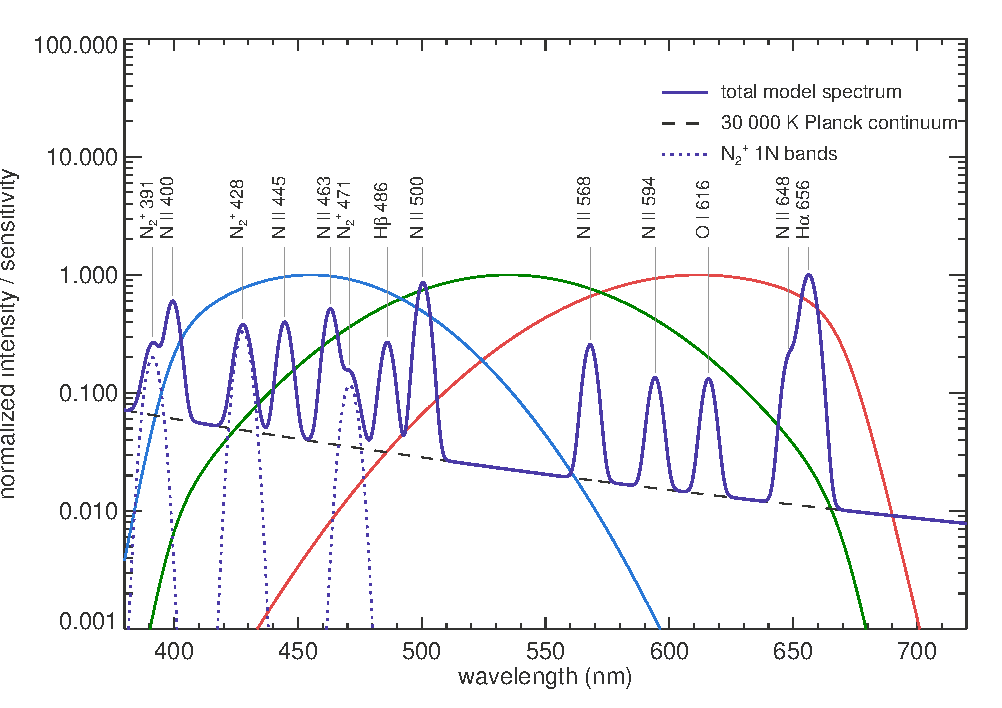
\includegraphics[width=\textwidth]{fig2a.pdf}
    \caption{}
  \end{subfigure}\hfill
  \begin{subfigure}[b]{0.345\textwidth}
    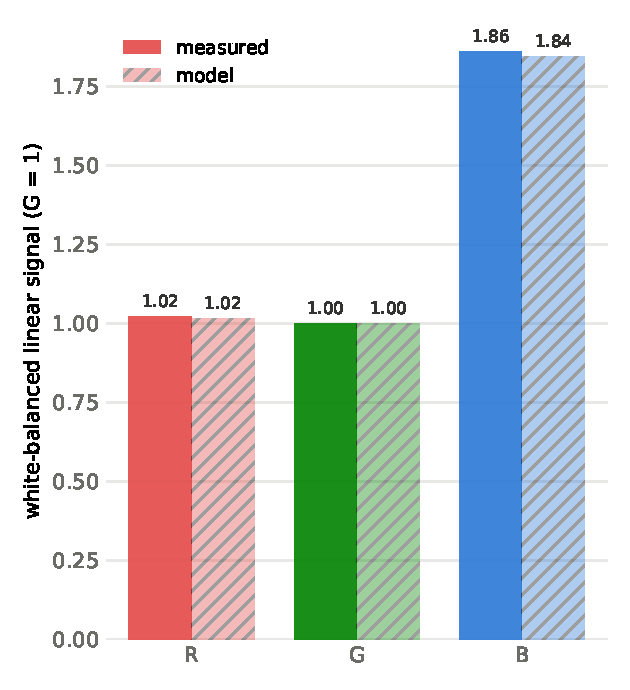
\includegraphics[width=\textwidth]{fig2b.pdf}
    \caption{}
  \end{subfigure}
  \caption{(a) The best-fit emission model on a log--linear scale, with
  every line labeled: the 30\,000~K Planck continuum (dashed), the \Ntp{}
  first-negative component (dotted), and the approximate camera channel
  sensitivities---red, green, and blue curves---including the 670~nm IR-cut
  edge (panel drawn in IDL~9.0). (b) Measured versus modeled white-balanced
  linear color, normalized to $G=1$.}
  \label{fig:spectrum}
\end{figure}

\subsection{Breaking the degeneracy}
\label{sec:degeneracy}
Three weights against two color ratios leave a one-parameter family: the
data cannot distinguish trading continuum against atomic-line energy, because
both are broadband compared to the camera channels. The degeneracy is not
fundamental, and several escapes are available, in roughly ascending order
of effort. \emph{(i) Priors.} Time-resolved spectrophotometry already bounds
the continuum share of visible stroke energy at the 10--25\% level
\citep{orville1968,orvillehenderson1984}; adopting that as a prior collapses
the family to $w_c\approx0.15$--0.25 without new hardware.
\emph{(ii) In-scene calibration.} The high-pressure-sodium streetlamps in
the same frame have a known, strongly structured spectrum (self-reversed
Na~D core plus scandium and mercury lines); photographing them---and a
reference color chart---through the production pipeline would measure the
effective channel curves and color matrix of this specific unit, removing
the systematic that currently dominates (\S\ref{sec:holes}), and tightening
the family. \emph{(iii) A fourth band.} Any additional, spectrally distinct
measurement over-determines the mixture: a second camera with different
(characterized) sensitivities, or two narrowband filters---one at 427.8~nm
for the molecular system, one at 656~nm for H$\alpha$---turn $w_m$ and the
H$\alpha$ amplitude into direct photometry. \emph{(iv) Time resolution.}
The components have distinct decay clocks: continuum and N\,\textsc{ii} die
in tens of microseconds, H$\alpha$ persists, molecular emission rides the
afterglow and any continuing current. Even 1000~fps video---1~ms bins---
would separate the hot-phase blend from the afterglow and split $w_c$ from
$w_a$ by lever arm on time rather than wavelength. \emph{(v) Ensembles.}
Across many flashes at varying (unknown) distances, the emission mixture is
approximately common while Rayleigh path-reddening scales with distance;
regressing observed colors across an ensemble separates source chromaticity
from propagation, calibrating the term we currently assume.
\emph{(vi) The grating.} A blazed transmission grating over a spare camera
makes the monitor a slitless spectrograph, and one storm's worth of frames
would replace this entire section with a measurement.

\section{Engineering: cloud, air, and silicon}
\label{sec:engineering}
\textbf{Water.} The flash reached the camera by diffusion through the
overcast deck. Cloud droplets ($\sim$10~$\mu$m) scatter visible light in the
geometric-optics regime with single-scatter albedo $\approx 1$ and negligible
wavelength dependence; multiple scattering randomizes direction and smears
time (by tens of microseconds per kilometer of diffusion path) but is nearly
chromatically neutral \citep{thomasonkrider1982,koshak1994,bohren1987}.
Liquid and vapor-phase water absorption in the visible is weak (the red-band
overtones are orders of magnitude too small over these path lengths). The
deck therefore acts as a large neutral diffuser: it preserves chromaticity
while converting a point stroke into hemispheric illumination---and, by
admixing multiply-scattered white light, desaturates it, which is why the
lavender is pale. We include one chromatic propagation term: Rayleigh
extinction over an assumed 3~km effective clear-air path,
$\tau(\lambda)=0.036\,(550/\lambda)^4$, a few-percent reddening.

\textbf{Silicon.} The camera (Elgato Facecam~4K, Sony STARVIS~2 sensor) is
operated with every automatic control disabled: manual exposure, manual
gain, white balance fixed at 5600~K. We model Bayer sensitivities as
Gaussians (B: 455/38~nm, G: 535/45~nm, R: 612/48~nm) within the family of
measured consumer-camera response functions \citep{jiang2013}, multiplied by
a 670~nm IR-cut and 398~nm UV edge; white-balance gains are defined so a
5600~K Planck source renders neutral. Because the WB is locked, the
$\sim$30\,000~K-class source renders honestly blue instead of being
neutralized---the instrumental design choice that makes this measurement
possible. Measured JPEG values are linearized with the sRGB transfer
function \citep{iec1999} and baseline-subtracted in linear space. The red
channel's retained sensitivity at 656~nm ($\sim$0.66 of peak) is what lets
H$\alpha$ lift $R$ to parity with $G$; a camera with an aggressive 650~nm
IR-cut would have rendered this flash noticeably bluer.

\section{Meteorology}
The synoptic context was a warm, saturated boundary layer: 100\% overcast at
2500--3000~m, 86--90\% surface humidity, with reanalysis showing drizzle
beginning exactly at the top of the hour \citep{hersbach2020}. No
thunderstorm code appears at the grid point---the flash likely came from an
isolated convective cell embedded in, or behind, the stratiform deck, of the
kind reanalysis routinely smooths away. Three faint blue excursions across
30 minutes suggest a small cell passing at distance. The wet-season
signature matters twice over: the humid air fed the H$\alpha$ line
(\S\ref{sec:physics}), and the low deck provided the projection screen. The
event is also a one-frame advertisement for fixed-exposure urban sky
monitoring: a 100~ms exposure every 300~s is a 1-in-3000 duty cycle, yet
over a season of nights even rare transients---lightning, fireworks,
aurora---will land in frames whose radiometry is interpretable after the
fact.

\section{N\,\textsc{ii}, \Ntp{}, and the ecosystem: the fertilizer in the
spectrum}
\label{sec:ecosystem}
The nitrogen spectrum of the flash is not just a curiosity; it points at
the atmosphere's strongest natural machine for breaking the N$\equiv$N
triple bond. That bond, at 9.8~eV, is why nitrogen---the most abundant
element in the atmosphere---is the limiting nutrient of most ecosystems:
molecular N$_2$ is biologically inert until something tears it open.
Lightning runs two factories that do, and our one pixel carries a
certificate from each.

The first factory is thermal, and its certificate is the \emph{atomic}
spectrum. Every N\,\textsc{ii} photon attests that an N$\equiv$N bond was
fully broken and the fragment ionized besides---and at $w_a\simeq0.6$ the
dissociation signal is not a garnish on the flash but most of its light.
The fixing, however, happens elsewhere, and in the dark. In the
$\sim$30\,000~K core nothing can be kept: nitric oxide formed there
re-equilibrates away. It is the 2000--4000~K cooling shell and mixing zone
that runs the Zel'dovich chain
($\mathrm{O_2 + N \rightleftharpoons NO + O}$ and its partner reaction),
freezing NO out of equilibrium as the gas cools
\citep{zeldovich1966,borucki1984}---and that shell is spectroscopically
silent: too cool to excite the visible N\,\textsc{ii} or near-infrared
N\,\textsc{i} lines, while the one low-lying transition of the crucial
metastable reagent, the [N\,\textsc{i}] 520~nm doublet of N($^2$D), is
collisionally quenched at tropospheric density (it is an aurora and
nightglow line precisely because it needs near-vacuum). The core that
shines does not fix; the shell that fixes does not shine.

The second factory is cold, and it is the one the violet bands advertise.
\Ntp{} is an intact molecule---ionization barely weakens the bond (order
2.5, 8.7~eV)---so a 427.8~nm photon certifies ionization, not
dissociation. But in cool plasma the dominant fate of \Ntp{} is
dissociative recombination, $\mathrm{N_2^+ + e^- \to N + N}$, branching
heavily to the metastable N($^2$D), whose reaction with O$_2$ yields
NO---the sequence that makes aurorae the nitric-oxide factory of the
thermosphere \citep{rees1989,barth1992}. That pathway operates exactly
where our molecular emission originates (the corona sheath, streamers, and
recombining afterglow, \S\ref{sec:molecular}), so the violet 12--21\% marks
a real if minority fixation channel: the opening move of the auroral
mechanism, running in the storm's cold plasma.

The budget belongs to the thermal factory. A single flash fixes of order
kilograms of nitrogen; globally, lightning contributes roughly
2--8~Tg~N~yr$^{-1}$, several percent of all natural fixation and the
dominant source of NO$_x$ in the free troposphere, where it regulates
ozone production \citep{borucki1984,schumann2007}. Before biological
nitrogenase evolved, such abiotic channels were the biosphere's nitrogen
supply; models of the Archaean atmosphere suggest declining CO$_2$ would
have throttled lightning fixation severely enough to constitute a nitrogen
crisis for early life \citep{navarrogonzalez2001}. The NO oxidizes to
NO$_2$---observed as column enhancements under storms since
\citet{noxon1976}---then to nitric acid, and rains out as nitrate. The
drizzle that began nineteen minutes after our frame carried that night's
nitrate down onto the lawns in the image foreground---the same lawns whose
green chromatic coordinate this instrument logs daily as a phenology
metric. The monitor, in one frame, photographed its own fertilization, and
the frame is signed by both factories in their budget order: two-thirds
atomic certificate, one-eighth-to-one-fifth violet.

\section{Aesthetics and color theory}
Lavender is a desaturated purple, and purple is the one hue family with no
spectral wavelength: it exists only as a ratio of the spectrum's two ends
against a deficit in the middle, on the line of purples that closes the CIE
diagram \citep{wyszecki1982}. That is precisely the spectrum lightning
supplies---nitrogen's violet and hydrogen's red bracketing a green
minimum---which is why lightning has read as violet to observers since long
before CCDs, and why daylight-balanced film renders it the same way
\citep{minnaert1954,salanave1961}. Goethe, wrong about mechanism and acute
about phenomenology, placed \emph{Purpur} at the summit of his color system:
the union of the two intensified poles of his polarity, a color nature
produces only under extremity \citep{goethe1810}. The lightning spectrum is
about as literal an enactment of that figure as physics offers---the two
ends of the visible conspiring against the middle.

The frame's beauty is relational, and here the French tradition earns its
keep. \citet{chevreul1839}, codifying simultaneous contrast for the Gobelins
dyers, showed that complementary colors mutually exalt one another; our
archive applies his law diachronically. The flash frame sits in a season of
sodium-amber nights (\code{\#1c1808}); amber and violet-blue are near
complements, so the anomalous frame does not merely differ from its
neighbors---it negates them, and each makes the other more vivid, the eye
carrying the remembered amber into the lavender. \citet{albers1963} made the
same point operational: color is never absolute, and the identical pixel
triplet pasted into a daylight scene would read as concrete grey.
\citet{wittgenstein1977} circles a related puzzle---whatever looks luminous
cannot look grey---and our sky obliges: values that would be a dull mauve on
paper look radiant solely because the surround is midnight. As for what the
photograph \emph{is}: in Barthes's terms the 5678 rows of the season's log
are \emph{studium}, and the one lavender row is \emph{punctum}, the detail
that pierces; his \emph{ça-a-été}---the photograph's stubborn
``that-has-been''---acquires an edge here, because this particular
that-has-been lasted 100~ms and was witnessed by no one
\citep{barthes1980}. \citet{merleauponty1945} held that color is not a
property but an encounter between a lived body and the world; this color
was encountered by an apparatus alone, and became a percept only in
retrospect, a memory without a rememberer. \citet{kandinsky1911} heard
violet as a cooled red, ``morbid, extinguished''---the thermodynamic pun is
free of charge---and \citet{pastoureau2000} reminds us violet served
centuries as \emph{demi-deuil}, half-mourning: for a tenth of a second, the
sky over Pittsburgh wore it.

\section{Holes in the theory}
\label{sec:holes}
In decreasing order of concern. (1)~\emph{The ISP is not sRGB.} The camera's
onboard pipeline applies a proprietary tone curve and color-correction
matrix; linearizing with the sRGB transfer function is an assumption, and a
CCM mixes channels post-hoc. The 1-DN agreement should therefore be read as
consistency, not precision. (2)~\emph{Three weights, two observables.} The
continuum--atomic split is unidentified; \S\ref{sec:degeneracy} lists the
escapes, none of which have yet been implemented. (3)~\emph{Channel
sensitivities are guessed Gaussians} within the plausible family
\citep{jiang2013}, not measurements of this unit; the H$\alpha$ leverage on
$R/G$ depends directly on the assumed red response at 656~nm and the IR-cut
edge. (4)~\emph{The continuum shape is bracketed, not known.} An earlier
version of this paper called the Planck-versus-recombination distinction
second order; fitting both limits (\S\ref{sec:fit}) shows it is first order
for the molecular weight ($w_m$ shifts from $\sim$0.13 to $\sim$0.19)
though not for any conclusion. The residual assumptions are that the
time-integrated continuum lies between the limits (a mixture of opacity
phases does) and that Gaunt factors and series edges smooth out over
100-nm-wide channels \citep{uman1965,zeldovich1966}. (5)~\emph{Line ratios are stroke-phase
averages}: a 100~ms exposure integrates hot early emission and the cool
afterglow in unknown proportion, and our literature amplitudes are typical,
not universal---flash type (intracloud versus cloud-to-ground), with
systematically different channel energetics \citep{rakovuman2003}, is itself
unknown. (6)~\emph{The propagation model is thin}: the 3~km Rayleigh path is
a guess, and in-cloud diffusion is taken as perfectly neutral. (7)~$n=1$,
8-bit quantization, JPEG compression, and the assumption that the amber
baseline adds linearly. Items (1) and (3) could be retired cheaply by the
in-scene calibration of \S\ref{sec:degeneracy}; item (5) invites the
grating.

\vspace{0.5em}
\noindent\textbf{Data.} The frame triplet, science log rows, fitting script,
and figure code (\code{fig2a.pro}, IDL~9.0; \code{lightning\_model.py}) are
archived with the monitor (\code{archive\_ref/2026-08-09/},
\code{science.csv}).

\begin{thebibliography}{29}

\bibitem[Albers(1963)]{albers1963}
J.~Albers, \emph{Interaction of Color} (Yale University Press, New Haven,
1963).

\bibitem[Barth(1992)]{barth1992}
C.~A. Barth, ``Nitric oxide in the lower thermosphere,'' \emph{Planet.\
Space Sci.} \textbf{40}, 315--336 (1992).

\bibitem[Barthes(1980)]{barthes1980}
R.~Barthes, \emph{La Chambre claire: Note sur la photographie}
(Gallimard/Seuil, Paris, 1980).

\bibitem[Bohren(1987)]{bohren1987}
C.~F. Bohren, ``Multiple scattering of light and some of its observed
consequences,'' \emph{Am.\ J.\ Phys.} \textbf{55}, 524--533 (1987).

\bibitem[Borucki and Chameides(1984)]{borucki1984}
W.~J. Borucki and W.~L. Chameides, ``Lightning: Estimates of the rates of
energy dissipation and nitrogen fixation,'' \emph{Rev.\ Geophys.\ Space
Phys.} \textbf{22}, 363--372 (1984).

\bibitem[Chevreul(1839)]{chevreul1839}
M.-E. Chevreul, \emph{De la loi du contraste simultan\'e des couleurs}
(Pitois-Levrault, Paris, 1839).

\bibitem[Goethe(1810)]{goethe1810}
J.~W. von Goethe, \emph{Zur Farbenlehre} (Cotta, T\"ubingen, 1810).

\bibitem[Hersbach et al.(2020)]{hersbach2020}
H.~Hersbach et al., ``The ERA5 global reanalysis,'' \emph{Q.\ J.\ R.\
Meteorol.\ Soc.} \textbf{146}, 1999--2049 (2020).

\bibitem[IEC(1999)]{iec1999}
IEC 61966-2-1:1999, \emph{Multimedia systems and equipment---Colour
measurement and management---Part 2-1: Default RGB colour space---sRGB}
(International Electrotechnical Commission, Geneva, 1999).

\bibitem[Jiang et al.(2013)]{jiang2013}
J.~Jiang, D.~Liu, J.~Gu, and S.~S\"usstrunk, ``What is the space of spectral
sensitivity functions for digital color cameras?'' in \emph{Proc.\ IEEE
Workshop on Applications of Computer Vision (WACV)}, 168--179 (2013).

\bibitem[Kandinsky(1911)]{kandinsky1911}
W.~Kandinsky, \emph{\"Uber das Geistige in der Kunst} (Piper, Munich, 1911).

\bibitem[Koshak et al.(1994)]{koshak1994}
W.~J. Koshak, R.~J. Solakiewicz, D.~D. Phanord, and R.~J. Blakeslee,
``Diffusion model for lightning radiative transfer,'' \emph{J.\ Geophys.\
Res.} \textbf{99}(D7), 14361--14371 (1994).

\bibitem[Merleau-Ponty(1945)]{merleauponty1945}
M.~Merleau-Ponty, \emph{Ph\'enom\'enologie de la perception} (Gallimard,
Paris, 1945).

\bibitem[Minnaert(1954)]{minnaert1954}
M.~Minnaert, \emph{The Nature of Light and Colour in the Open Air}
(Dover, New York, 1954).

\bibitem[Navarro-Gonz\'alez et al.(2001)]{navarrogonzalez2001}
R.~Navarro-Gonz\'alez, C.~P. McKay, and D.~Nna Mvondo, ``A possible nitrogen
crisis for Archaean life due to reduced nitrogen fixation by lightning,''
\emph{Nature} \textbf{412}, 61--64 (2001).

\bibitem[Noxon(1976)]{noxon1976}
J.~F. Noxon, ``Atmospheric nitrogen fixation by lightning,'' \emph{Geophys.\
Res.\ Lett.} \textbf{3}, 463--465 (1976).

\bibitem[Orville(1968)]{orville1968}
R.~E. Orville, ``A high-speed time-resolved spectroscopic study of the
lightning return stroke, Parts I--III,'' \emph{J.\ Atmos.\ Sci.}
\textbf{25}, 827--856 (1968).

\bibitem[Orville and Henderson(1984)]{orvillehenderson1984}
R.~E. Orville and R.~W. Henderson, ``Absolute spectral irradiance
measurements of lightning from 375 to 880 nm,'' \emph{J.\ Atmos.\ Sci.}
\textbf{41}, 3180--3187 (1984).

\bibitem[Pastoureau(2000)]{pastoureau2000}
M.~Pastoureau, \emph{Bleu: Histoire d'une couleur} (Seuil, Paris, 2000).

\bibitem[Prueitt(1963)]{prueitt1963}
M.~L. Prueitt, ``The excitation temperature of lightning,'' \emph{J.\
Geophys.\ Res.} \textbf{68}, 803--811 (1963).

\bibitem[Rakov and Uman(2003)]{rakovuman2003}
V.~A. Rakov and M.~A. Uman, \emph{Lightning: Physics and Effects}
(Cambridge University Press, Cambridge, 2003).

\bibitem[Rees(1989)]{rees1989}
M.~H. Rees, \emph{Physics and Chemistry of the Upper Atmosphere}
(Cambridge University Press, Cambridge, 1989).

\bibitem[Salanave(1961)]{salanave1961}
L.~E. Salanave, ``The lightning spectrum as measured by slit and slitless
spectrographs,'' \emph{Science} \textbf{134}, 1395--1399 (1961).

\bibitem[Salanave et al.(1962)]{salanave1962}
L.~E. Salanave, R.~E. Orville, and C.~N. Richards, ``Slitless spectra of
lightning in the region from 3850 to 6900 angstroms,'' \emph{J.\ Geophys.\
Res.} \textbf{67}, 1877--1884 (1962).

\bibitem[Schumann and Huntrieser(2007)]{schumann2007}
U.~Schumann and H.~Huntrieser, ``The global lightning-induced nitrogen
oxides source,'' \emph{Atmos.\ Chem.\ Phys.} \textbf{7}, 3823--3907 (2007).

\bibitem[Thomason and Krider(1982)]{thomasonkrider1982}
L.~W. Thomason and E.~P. Krider, ``The effects of clouds on the light
produced by lightning,'' \emph{J.\ Atmos.\ Sci.} \textbf{39}, 2051--2065
(1982).

\bibitem[Uman and Orville(1964)]{uman1964}
M.~A. Uman and R.~E. Orville, ``Electron density measurement in lightning
from Stark-broadening of H$\alpha$,'' \emph{J.\ Geophys.\ Res.}
\textbf{69}, 5151--5154 (1964).

\bibitem[Uman and Orville(1965)]{uman1965}
M.~A. Uman and R.~E. Orville, ``The opacity of lightning,'' \emph{J.\
Geophys.\ Res.} \textbf{70}, 5491--5497 (1965).

\bibitem[Wallace(1964)]{wallace1964}
L.~Wallace, ``The spectrum of lightning,'' \emph{Astrophys.\ J.}
\textbf{139}, 994--998 (1964).

\bibitem[Wittgenstein(1977)]{wittgenstein1977}
L.~Wittgenstein, \emph{Bemerkungen \"uber die Farben / Remarks on Colour},
ed.\ G.~E.~M. Anscombe (Blackwell, Oxford, 1977).

\bibitem[Wyszecki and Stiles(1982)]{wyszecki1982}
G.~Wyszecki and W.~S. Stiles, \emph{Color Science: Concepts and Methods,
Quantitative Data and Formulae}, 2nd ed.\ (Wiley, New York, 1982).

\bibitem[Zel'dovich and Raizer(1966)]{zeldovich1966}
Ya.~B. Zel'dovich and Yu.~P. Raizer, \emph{Physics of Shock Waves and
High-Temperature Hydrodynamic Phenomena} (Academic Press, New York, 1966).

\end{thebibliography}

\end{document}
